\section{机制设计}

星云聚焦链上治理,致力于运用区块链技术来提供更公平的协作环境。

\subsection{链上治理流程}
\label{governance}

星云链上治理通用流程如图~\ref{fig:on-chain-governance}:

\begin{enumerate}
	\item \textbf{提案阶段}(Proposal Period):发起人在社区公开发起提案,在提案投票期间,如果通过了NAT链上投票,则项目立项;
	\item \textbf{执行阶段}(Develop Period):项目立项,提案人本人或经本人认可的社区成员按计划执行;
	\item \textbf{公测阶段}(Testing Period):执行人提交结果,在公测投票期间,如果通过了NAT链上投票,则进入下一阶段;
	\item \textbf{发布阶段}(NBRE Period):通过了两次投票的项目,社区没有异议且经技术委员会验收核实,即可最终执行发布。
\end{enumerate}

\begin{figure}
	\centering
	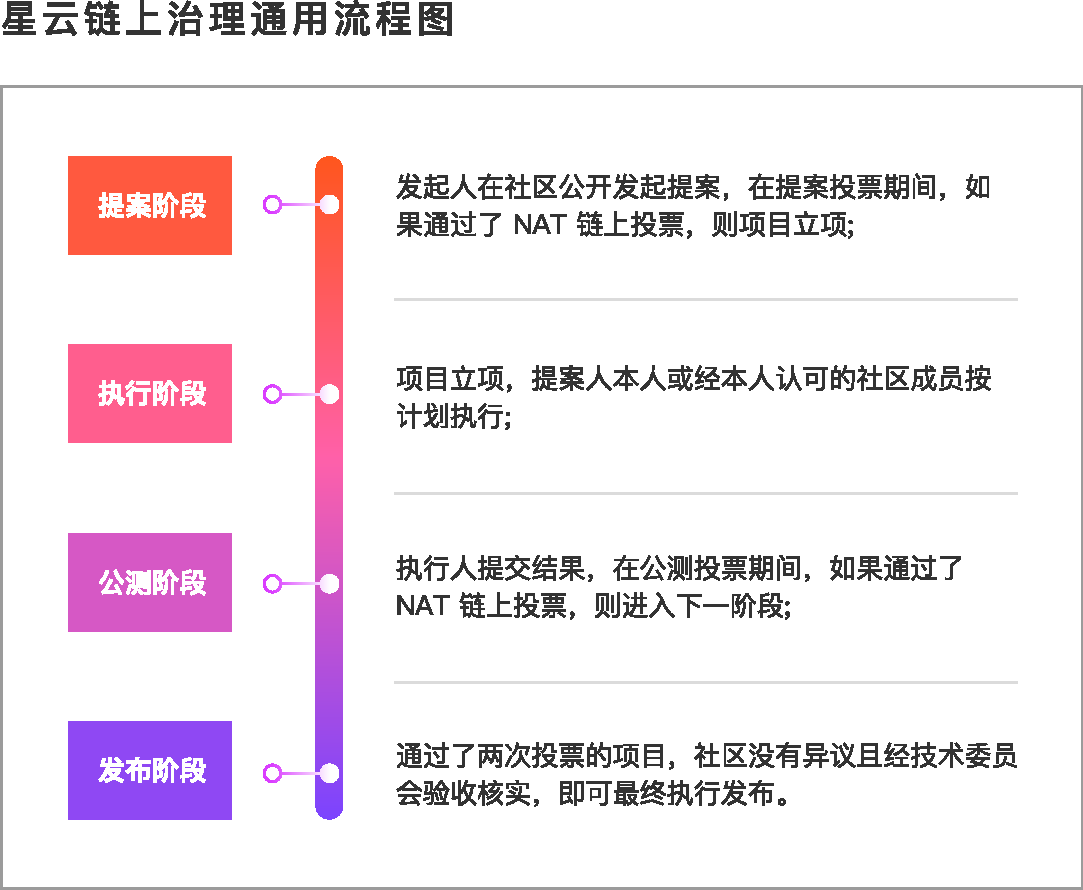
\includegraphics[width=1\textwidth]{../common/ch/on-chain-governance.pdf}
	\caption{星云链上治理通用流程图 \label{fig:on-chain-governance}}
\end{figure}

其中,“NAT链上投票”是核心手段,包括两部分:

\begin{enumerate}
	\item 投票唯一介质:NAT及其底层算法是星云链上治理的重要工具;
	\item 链上投票流程。
\end{enumerate}

本章节将对其进行重点介绍。

\subsection{投票基本原则}

星云生态通过星云主网实现链上投票。社区投出的每一票,将在星云链的区块上公开透明地展现。在星云链的系统中,投票将遵循以下基本原则:

\begin{enumerate}
	\item 投票的最基本单位是一个星云主网地址。
	\item 星云链的投票权重将参照地址的星云指数。
	\item 对系统有积极贡献的行为应被奖励更多的投票权,在投票的场景中,我们认为投票行为是对星云系统有积极贡献的行为,应被激励更多的投票权。
\end{enumerate}

\subsection{投票方式}

投票将通过星云主网上的投票智能合约实现,每个地址可以选择投赞同、反对、弃权三种票。亦可不参与投票。

\subsection{投票唯一介质:NAT}
\label{nat}

\subsubsection{概述}

\begin{itemize}
	\item \textbf{名称:} Nebulas Autonomous Token
	\item \textbf{代号:} NAT
	\item \textbf{形式:} NRC20 token
\end{itemize}

NAT是星云指数的资产形态,它以NRC20 Token的形式体现,并作为星云生态治理场景中唯一的投票介质。

\begin{center}
\fboxsep24pt
\colorbox{yellow!30}{
\begin{minipage}[c]{.8\textwidth}
	\paragraph{什么是星云指数?}
	星云指数是首个衡量区块链多维数据的价值标准,是星云核心的排序算法。

	在星云经济体中,治理的基本单位是一个\emph{地址}(参见\ref{rights})。星云指数通过对每个地址贡献度的数学表达,量化了每个“\emph{个体}”对于经济总量的贡献。星云指数分为\emph{核心星云指数}和\emph{扩展星云指数}(Extended Nebulas Ranks)。其中,核心星云指数受两个因素影响:

	\begin{enumerate}
		\item 账户在一定时期内的资产中值;
		\item 账户在一定时期内的出入度衡量。
	\end{enumerate}

	在宏观层面,核心星云指数使用经济学中经典的货币数量方程描述了区块链中货币数量、货币价值和流通速率以及生产力几者之间的关系。因此,全网的核心星云指数可以反映星云生态整体的流通性和活跃度。

	\paragraph{NAX和质押关系?}

	NAT的发行主要参考“\emph{核心星云指数}”,是核心星云指数的资产表现,NAT发行将以周为单位,参考一周之内地址的资产中值和出入度衡量计算所得的星云指数。关于星云指数的更多信息,请参考2018年6月星云研究院发布的《星云指数黄皮书》。

	\paragraph{如何查询?}

	星云指数在2019年5月6日Nebulas NOVA~\cite{nova}完成第一次投票升级后上链,可以通过Nebulas NOVA的核心能力星云区块链可执行环境(Nebulas Blockchain Runtime Environment,NBRE)实现升级。核心星云指数开源,可在线查询~\cite{CheckNR}。

\end{minipage}}
\end{center}

\subsubsection{应用场景}

NAT是星云治理中,链上投票场景的唯一介质,支持星云推进社区的治理。社区成员可以通过NAT进行链上投票表达自己对星云生态的意见,包括但不限于星云理事会的选举、星云主网通过星云区块链可执行环境(NBRE)执行星云协议表示(Nebulas Protocol Representation,NRR)、社区提案的立项、项目成果公测等。

\subsubsection{发行}
	
NAT的发行方式和比特币类似,在总量存在上限的前提下,按一定周期内全网星云指数的情况,以周为单位递减释放。

NAT协议的数量上限和星云链主网的全网星云指数值相关,释放量按周递减。递减系数为:$\lambda$。初始数值$\lambda$=0.997,即约在第180周时,发行量递减为第一周的58\%。

NAT的初始发行量以2019年5月6日星云主网Nebulas NOVA完成第一次投票升级后的全网星云指数为参照。假设全网星云指数和初始参数不变,NAT初始总量上限为1,000亿枚。

\subsubsection{管理NAT}

用户可以在NAS nano Pro~\cite{NASnano}及其他支持NRC20的客户端中~\cite{wallets}管理自己的NAT。同时,用户可以在支持星云链的区块链浏览器~\cite{explorer}上查看NAT的交易、流通情况等。

\subsection{获取NAT}

所有拥有星云主网地址的用户均有机会获得NAT。除黑名单地址外,星云主网地址的用户可以通过提升地址的星云指数、参与星云主网链上投票,或质押NAS三种方式获得NAT。


\paragraph{NAT的黑名单地址}

在NAT的发行过程中,与星云“\emph{地址}”基本权利主张(参见~\ref{rights})任何一条产生冲突的地址将被归为黑名单地址。黑名单地址只能根据其享有的权利获得部分NAT。

例如中心化交易所的地址就被归为黑名单地址。依照星云地址第一点基本权利主张,该地址具备拥有和操作星云链上资产的权利,所以交易所的归集地址可以在同等条件下按照地址的星云指数获得NAT,但这部分NAT的产权应属于对应的交易所用户。依照星云地址第二、第三点基本权利主张,在交易所证明该归集地址充分代表了相应托管资产用户提案和投票意愿之前,交易所归集地址并不具备发起提案和参与提案投票的权利,因此亦不能通过参与投票获得投票部分的NAT激励。


\subsubsection{通过提升地址的星云指数获得NAT}

对于有星云指数的地址,NAT协议将按周向该地址进行发放,发放的数量将参照该地址上一周的星云指数和星云全网星云指数的情况。

对于有星云指数的地址,每周获得NAT的数量递减,递减系数为$\lambda$。初始数值$\lambda$=0.997。

在第$i$周,获得NAT的比例约为:

\begin{align}
1\,\text{NR}=z(x_{ne},x_{e},\mu)\times\lambda^{i}\,\text{NAT}
\end{align} 

其中:
\begin{itemize}
	\item $\lambda$:衰减系数;
	\item $\mu$:投票行为的激励参数;
	\item $x_{ne}$:全网非交易所地址的星云指数总和;
	\item $x_{e}$:全网交易所地址的星云指数总和;
	\item $z(x_{ne},x_{e},\mu)$:以$x_{ne}$、$x_{e}$和$\mu$为变量的函数,星云指数和NAT的兑换比例。
\end{itemize}

\subsubsection{通过质押星云链主网原生代币(NAS)获得NAT}

从2019年5月6日开始,星云主网地址用户可以选择向投票的智能合约质押星云主网原生代币星云币(NAS)获得NAT。

质押NAS的用户将从质押开始后的第2周(即不早于2019年5月13日)开始获得NAT。如果用户取回质押的NAS,则停止获得NAT。

质押NAS的用户每周获得NAT的数量递减,递减系数为$\lambda$,初始数值$\lambda$=0.997,

第$i$周质押NAS获得NAT的比例为: 

\begin{align}
x \text{NAS} \rightarrow \alpha \times z(x_{ne},x_{e},\mu)\times g(x) \times \lambda^{i} \text{NAT}
\end{align}

其中:

\begin{itemize}
	\item $x$:质押NAS的数量;
	\item $\alpha$:质押系数,初始数值$\alpha$=5;
	\item $z(x_{ne},x_{e},\mu)$:以$x_{ne}$、$x_{e}$和$\mu$为变量的函数,星云指数和NAT的兑换比例;
	\item $g(x)$:与$x$相关的函数,用于模拟以$x$值的NAS在星云主网获得的星云指数的情况。
\end{itemize}

\vspace{2em}

\textbf{如何发起质押?} 
	
用户可以通过使用星云钱包NAS nano Pro或其他支持NAS的客户端向投票智能合约发送交易,确认要质押NAS的数量。

为了保证用户可以获得并管理NAT,用户需要用自己掌握私钥的主网地址向星云的投票智能合约发送NAS完成质押,请勿使用交易所账户发送交易。

\vspace{2em}

\textbf{如何取消质押?}

用户可以通过NAS nano Pro或其他客户端调用智能合约申请取消,取消后可立即取回质押的NAS,取消质押后,则停止获得NAT。

\subsubsection{通过参与星云链上投票获得NAT}

星云主网地址获得了NAT后,可以选择参与或不参与社区治理链上投票。在此次投票周期中,如果用户参与了投票,无论投出赞成、反对还是弃权票,均可获得投票激励。如果未参与投票,则无法获得激励。

\vspace{2em}

\textbf{激励规模}

我们认为激励的规模应该是适当的,不应该被恶意使用。投票的激励会取决于:

\begin{enumerate}
	\item 该地址当周所投NAT的数量;
	\item 该地址上一周星云指数及该星云指数对应可获得的NAT。
\end{enumerate}

当用户投出符合自己地址星云指数对应的NAT会得到激励,如果用户投出的NAT超过自己地址星云指数对应的NAT,超出部分将无法获得激励。
	
第$i$周,参与链上投票的地址获得的激励规模为:

\begin{align}
\mu\times \min\{N_{v},N_{nr}\}  \times \lambda^{i}
\end{align}

其中:

\begin{itemize}
	\item $\mu$:激励系数,初始数值$\mu$=10;
	\item $\lambda$:递减系数,初始数值$\lambda$=0.997;
	\item $N_{v}$:当周该地址投出的NAT数额;
	\item $N_{nr}$:该地址上一周的星云指数对应可获得的NAT。
\end{itemize}

即,当该地址当周投出的$N_{v}$小于或等于$N_{nr}$的时候,获得的激励数量为$\mu\times Nv$,当该地址当周投出的$N_{v}$大于$N_{nr}$的时候,获得的激励数量为$\mu\times N_{nr}$。

举例来说,假如某个地址根据上一周的星云指数值获得了10 NAT,该地址上一共有1,000 NAT,如果当周该地址投出了5 NAT,小于该地址上一周星云指数对应可获得的NAT数值(10 NAT),故将获得$10\times5=50$ NAT投票激励。如果该地址投出了1,000 NAT,超出10 NAT,则将获得$10\times10=100$ NAT投票激励。

和提升星云指数获得NAT及质押NAS获得NAT一样,通过投票激励获得的NAT也是按周递减的,递减系数为$\lambda$,初始数值$\lambda$=0.997。

\subsection{投票规则}
	
\subsubsection{投票手续费}

每次投票将收取$\theta$\% NAT将作为投票手续费,此部分手续费由星云理事会授权交由星云基金会作为NAT项目的专项运营资金管理,项目团队不得将此部分手续费直接用于投票。初始数值$\theta$=3。

\subsubsection{投票和NAT销毁}

在每个发行周期内,用户投入星云链投票智能合约的NAT将被立即销毁,销毁的比例会按照周期递减,递减速率和NAT发行的递减速率一致。每个周期内销毁部分的NAT将按照NAT销毁速率函数计算,具体公式参见附录\ref{burn}。

\subsubsection{投票通过标准}
	
投票是否通过将通过两个维度的标准来衡量:投票的参与度和赞成票的占比。

\begin{enumerate}
	\item 

	\textbf{投票参与度:}

	对于涉及到使用公共资产支持的提案,投票的参与度不得低于该提案提起资产占全网流通资产的比例。

	如某提案要求动用$X$ NAS支持,此时星云主网中流通的NAS(任何未在锁仓/质押状态、可随时在星云主网上进行转账交易的NAS)为$Y$。

	则此提案通过需要达成的全网投票参与度不得低于$X/Y$,换算成NAT来表示,及参与此次投票的NAT与该周期初期给用户的NAT的比例不得低于$X/Y$。

	对于不涉及到使用公共资产支持的提案,投票的参与度由社区共同决定,此类提案包括但不限于星云主网参数的调整、NBRE要执行的NPR等。

	\item

	\textbf{赞成票的占比:}

	在满足投票最低参与度之外,某一提案投票是否通过还需要满足赞成票占总投入票数的比例不得低于51\%。

	即假设某一提案共收到票数为N,其中赞成票为Y,反对票为N,弃权票为A,则只有当$Y/(Y+N+A) \ge 51\%$时,此提案才被视为投票通过。
\end{enumerate}

\subsection{投票监督和管理}

\subsubsection{投票流程监督}
\label{second-vote}

星云技术委员会受星云理事会委任,负责监督治理流程,保证整个流程公开透明。星云社区链上公开投票由星云技术委员会负责组织和管理。

公开投票接受社区所有成员的公开监督。针对违反星云基本权利主张的提案,星云技术委员会可以向星云理事会发起重审提案申请。星云理事会作为星云生态中治理流程正当性的监督者,有权对某一提案提起且仅能提起一次进行“\textbf{二次投票}”的要求。

当理事会提出“二次投票”的要求时,该提案被视为进入到新的投票周期进行一次新的投票。第一次投票过程中的结果不被执行,第一次投票投出的NAT不予返还,会按照当周期的烧毁速率进行烧毁。

二次投票的投票参与度需大于第一次投票的参与度。即假设第一次投票的参与度为$X/Y$,则第二次投票的参与度应大于$X/Y$,且赞成票的比例不低于51\%,方可视为投票通过。

\subsubsection{NAT参数调整}

NAT的发行过程涉及到如下系数:

\begin{enumerate}
	\item $\alpha$:质押系数,初始数值$\alpha$=5
	\item $\mu$:投票奖励系数,初始数值$\mu$=10
	\item $\lambda$:递减系数,初始数值$\lambda$=0.997
	\item $\theta$:投票手续费,初始数值$\theta$=3
\end{enumerate}

系数的调整需要经过星云生态的治理投票流程,星云基金会或NAT项目团队无权擅自调整系数。




